\section{Methods}

\subsection{Photographic Technique}
% Must be a more technical name for this - nailed it

As per the PhotoScan user
manual\footurl{http://downloads.agisoft.ru/pdf/photoscan-pro_1_0_0_en.pdf}, the
photos were taken at an oblique angle to the object being modelled (namely the
ground). This amount to ensuring that the camera is facing down towards the
ground. This is illustrated in Figure \ref{img:photographic-method}.

\begin{figure}[H]
    \centering
    \begin{subfigure}[b]{0.49\textwidth}
        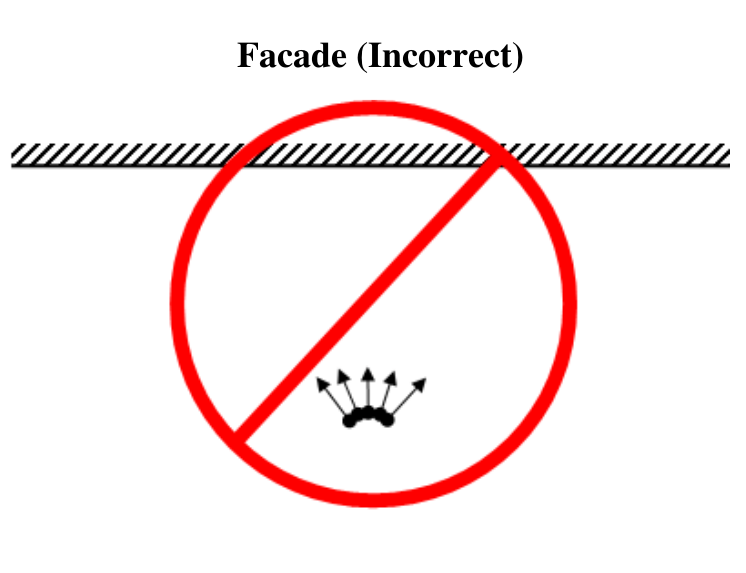
\includegraphics[width=\textwidth]{Incorrect}
        \label{img:incorrect}
    \end{subfigure}
    \begin{subfigure}[b]{0.49\textwidth}
        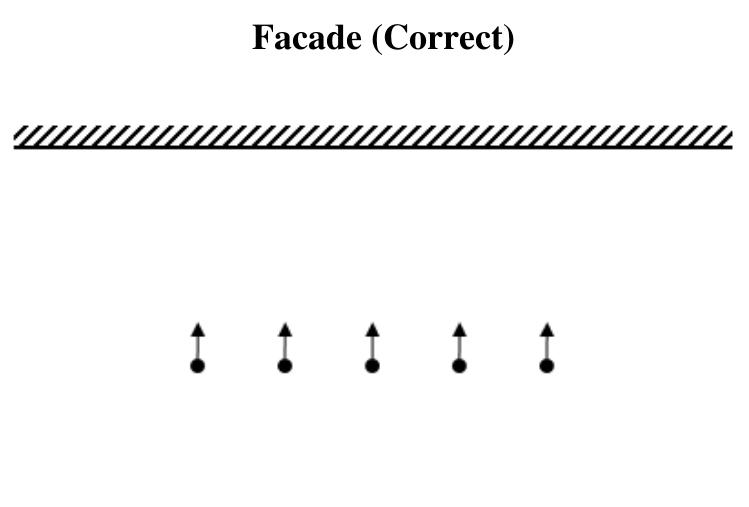
\includegraphics[width=\textwidth]{Correct}
        \label{img:correct}
    \end{subfigure}
    \caption{The incorrect and correct method of taking photos useful for
        photogrammetric modelling, reproduced from the
        \href{http://downloads.agisoft.ru/pdf/photoscan-pro\_1\_0\_0\_en.pdf}{Agisoft
        PhotoScan User Manual, Version 1.0}}
    \label{img:photographic-method}
\end{figure}

\subsection{CHDK Scripts}

\subsubsection{Time Interval}

The method used predominantly for remote photography is to run a script which
automatically takes photos after a regular interval specified by the user. The
Lua script for this can be found in Appendix \ref{app:interval}. To ensure that
the photos take at regular intervals, we tested the actual time between
photographs, at different input interval values. The results, illustrated in
Figure \ref{fig:camera-timing}, show that below 5 seconds the interval is
unreliable. We therefore used 5 seconds as the standard time interval between
photos.

\begin{wrapfigure}{r}{0.5\textwidth}
    \centering
    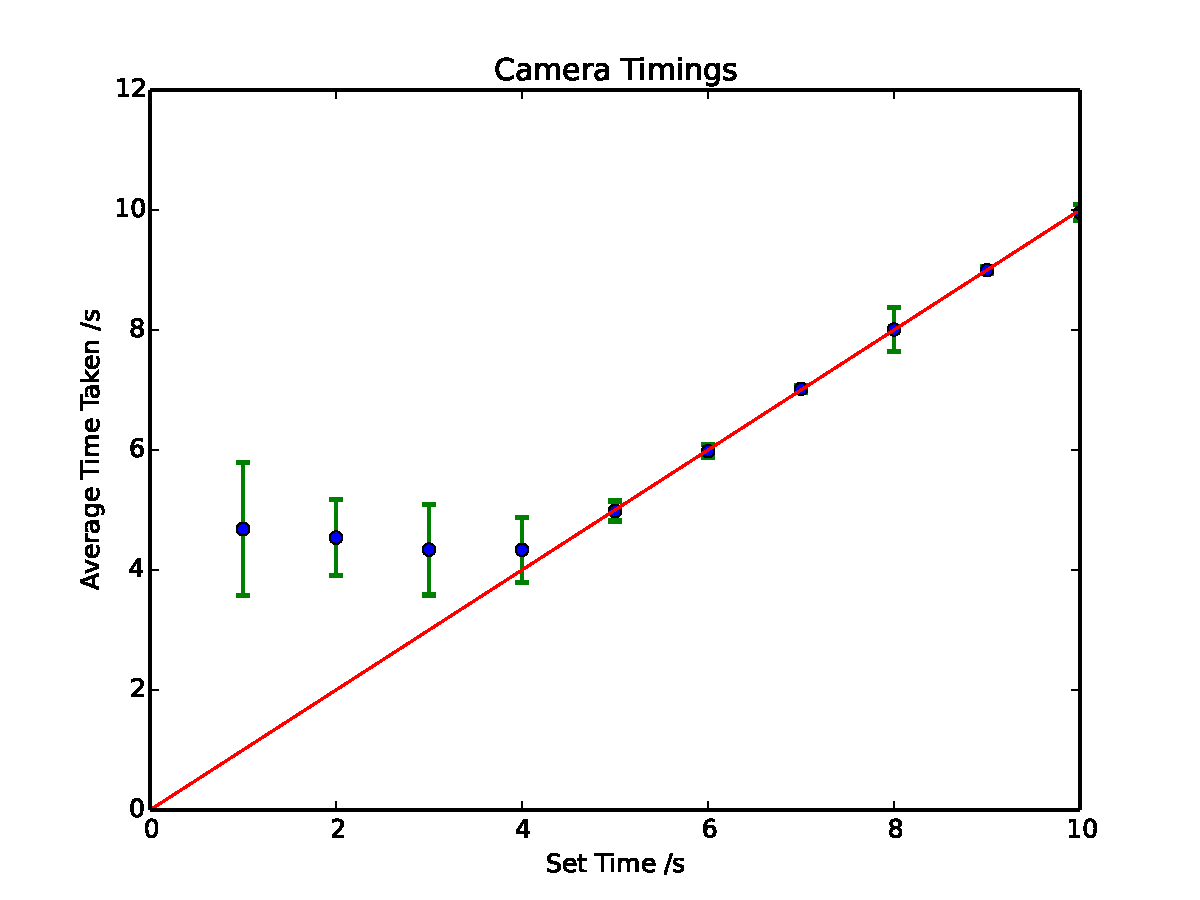
\includegraphics[width=0.5\textwidth]{CameraTiming}
    \caption{The measured averaged time difference between successive photos,
        plotted against the interval input into the script. 11 photos, giving
        10 time differences, were taken.}
    \label{fig:camera-timing}
\end{wrapfigure}

\subsubsection{Pulse Width Modulation Signal}

Although it is not used for this research, CHDK scripts can take advantage of
the \texttt{get\_usb\_power} function to take input from APM. This utilises
Pulse Width Modulation (PWM), whereby repeated short digital signals are
interpreted as different voltages due to their high frequency. The APM autipilot
send these PWM signals to the camera via a cable, pictured in Figure
\ref{img:chdk-cable}, where the camera interprets them as different voltages.
The CHDK script that interprets these voltages, written in UBASIC, is given in
Appendix \ref{app:pwm}.

Note that the \texttt{Enable Remote} parameter must be enabled under
\texttt{Settings} $\rightarrow$ \texttt{CHDK Settings} $\rightarrow$
\texttt{Remote Parameters}.

\begin{wrapfigure}{r}{0.5\textwidth}
    \begin{center}
        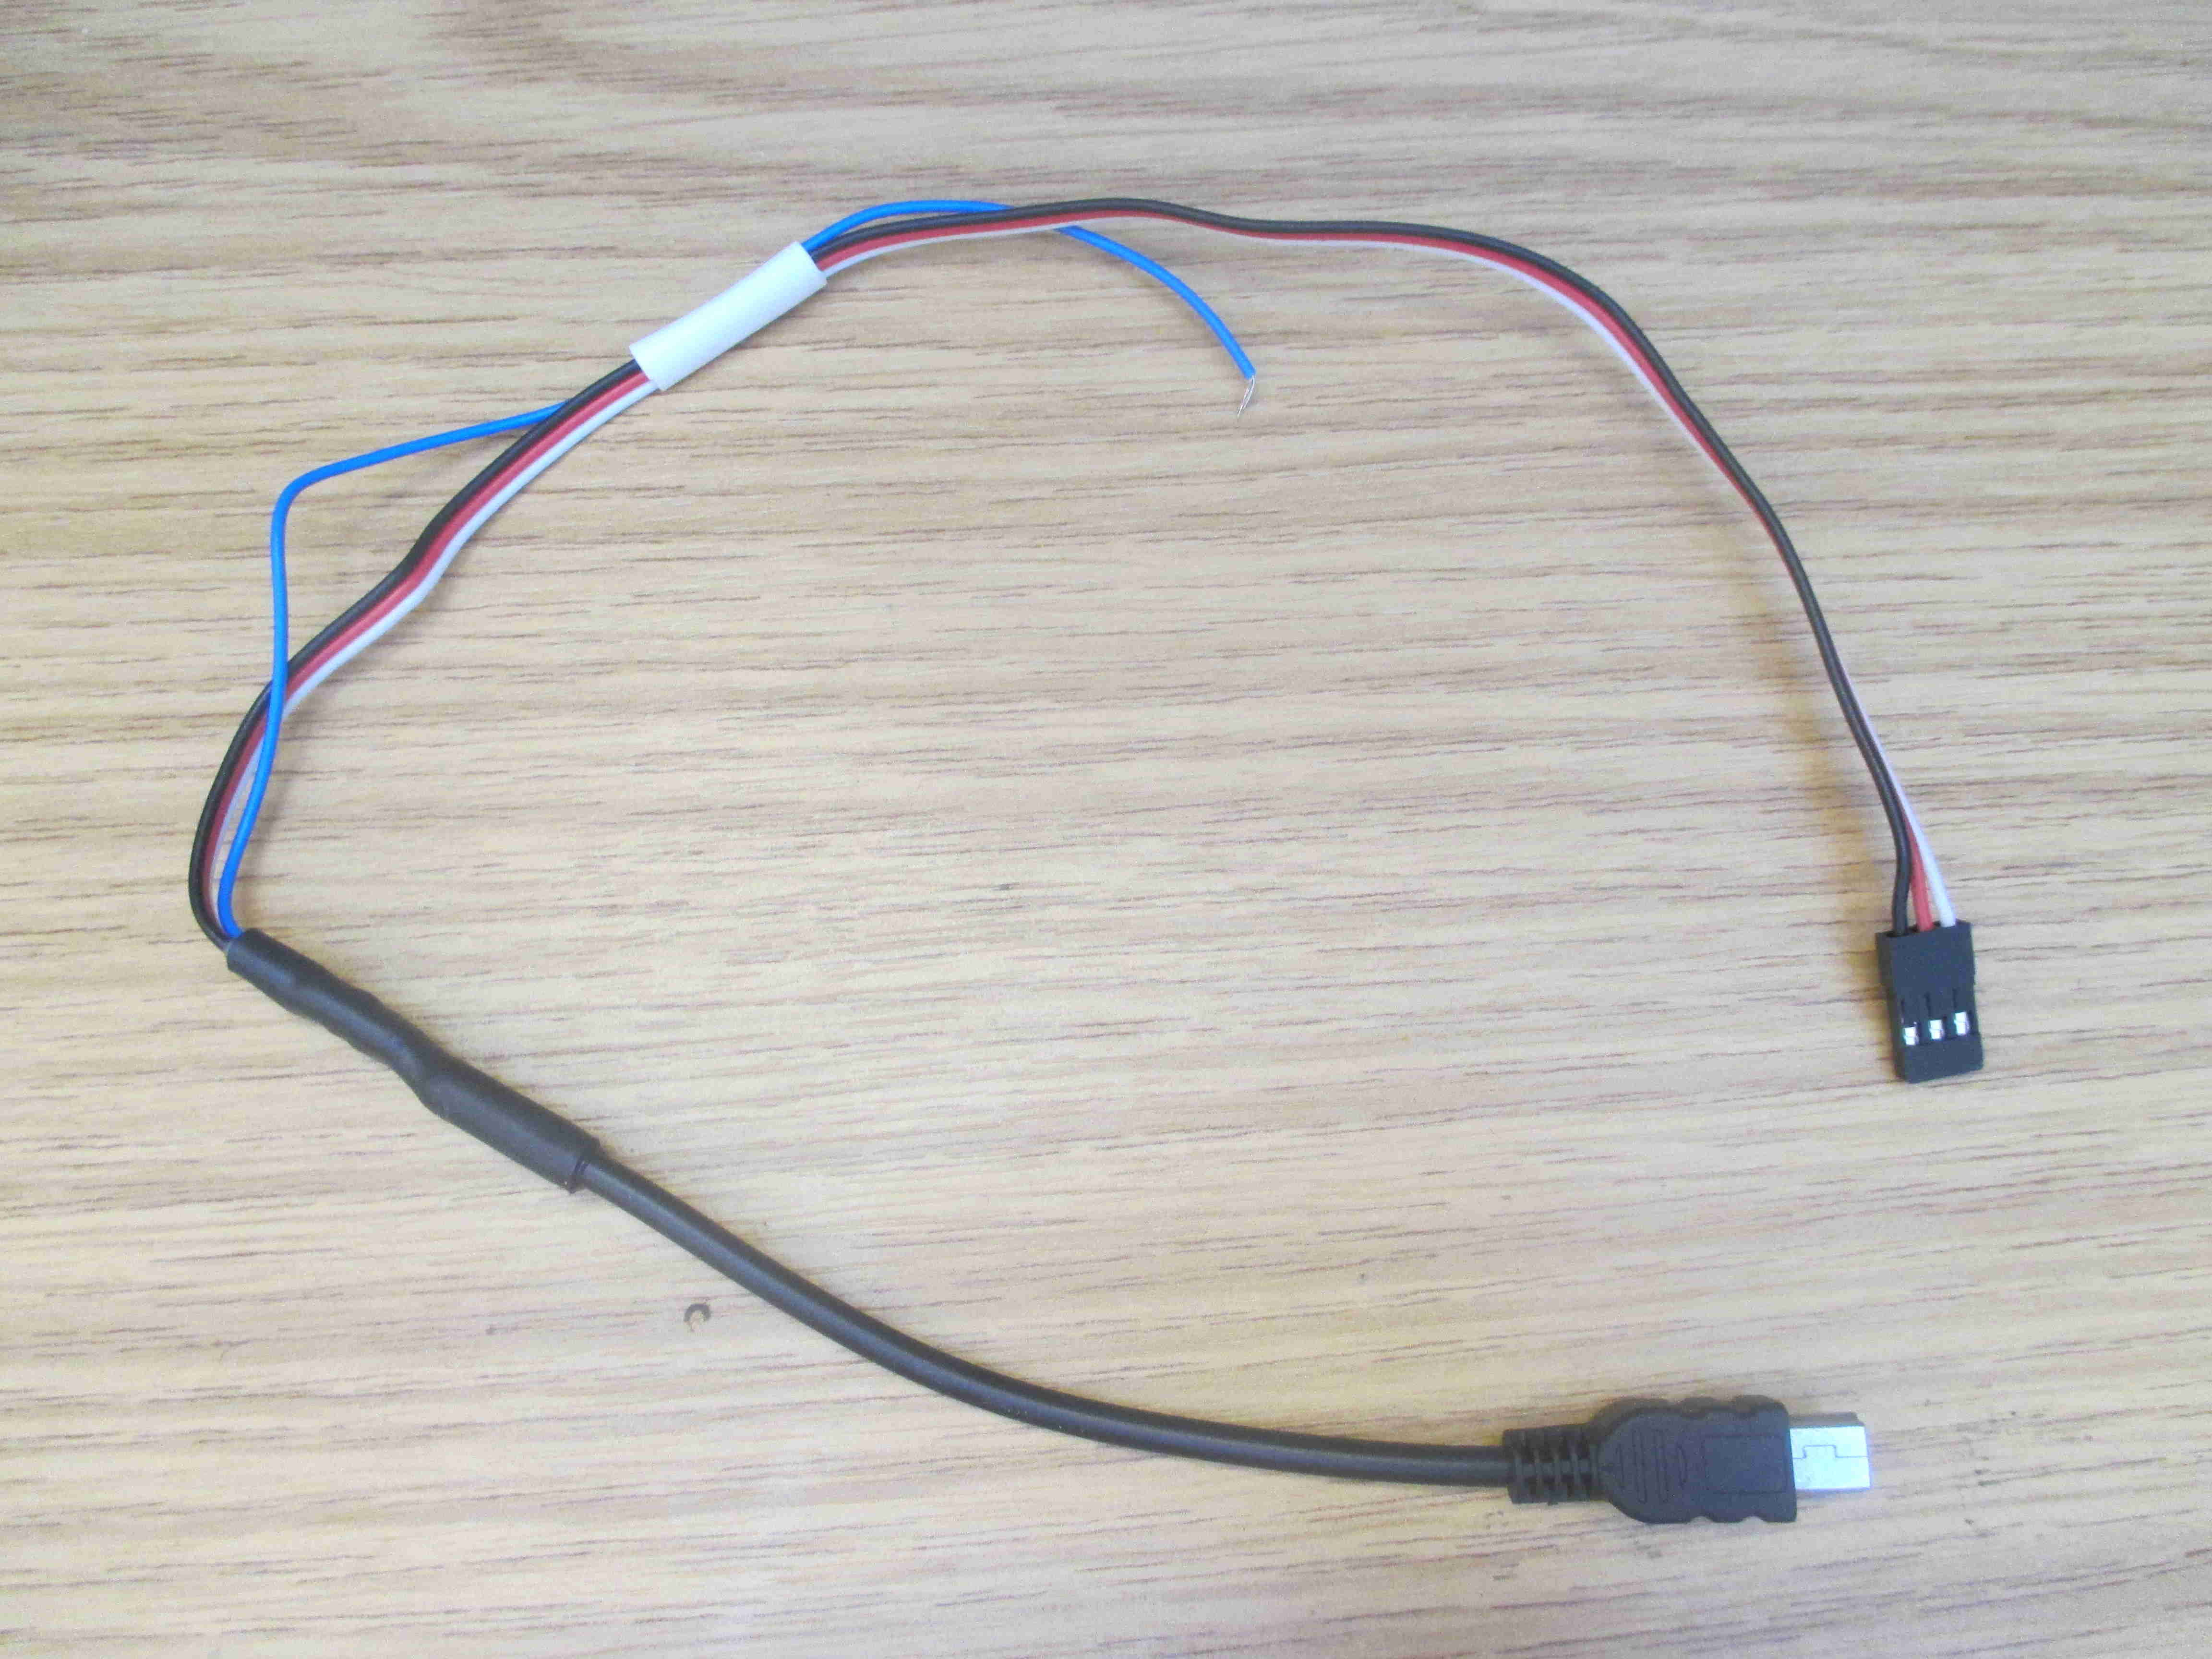
\includegraphics[width=0.5\textwidth]{CHDKCable}
        \caption{The cable used to connect the camera running CHDK to the APM board.
            PWM signals are sent through this cable and interpreted by scripts
            running on the camera}
        \label{img:chdk-cable}
    \end{center}
\end{wrapfigure}

Using the time interval script is in general more practical than taking photos
through the CHDK cable using PWM. This is because the time interval method is as
Isimple as strapping the camera to the copter and setting to photographing,
whereas when using the CHDK cable, one needs to either set APM to take photos at
every waypoint using MP, which one cannot do when controlling the UAV manually,
or assign the camera `shoot' functionality to a button on the radio control
system, in which case one needs to press this button every few seconds.

\subsection{Geotagging}
\label{sec:methods/geotagging}

In order to increase the accuracy and precision of the camera location in the
photogrammetry software, and thereby the accuracy and precision of the final
model, the photos are tagged with their location by using the UAV's on-board
Global Positioning System (GPS). The geolocation is written either into a
separate comma separated value (CSV) file, or is written directly into the exif
metadata of the photos themselves. Either can be imported into PhotoScan. The
technique used to determine the location of the photographs depends on whether
the photographs were taken using the time interval script or as controlled by
the APM autopilot.

\subsubsection{Time Offset Method}

If the camera is set to automatically take pictures every 5 seconds, then one
needs to know the difference between the internally logged time on the camera,
stamped onto the photographs' exif metadata by the camera automatically, and the
GPS time on the UAV. As the UAV constantly takes logs of its GPS location and
the time, knowing the time difference between camera and GPS is sufficient to
determine the location of each of the photos. Inputting the log, photographs and
time difference into MP, MP automatically geotags the photos to be imported into
PhotoScan.

In order to find this time difference, a photograph of MP while connected
directly by USB to the APM, as illustrated in Figure \ref{img:mission-planner},
is taken. As the UAV GPS time is displayed on the MP screen, and the camera logs
the time it takes the photograph, comparing the exif time stamp to the GPS time
recorded in the photo itself gives the time difference.

\begin{wrapfigure}{r}{0.5\textwidth}
    \begin{center}
        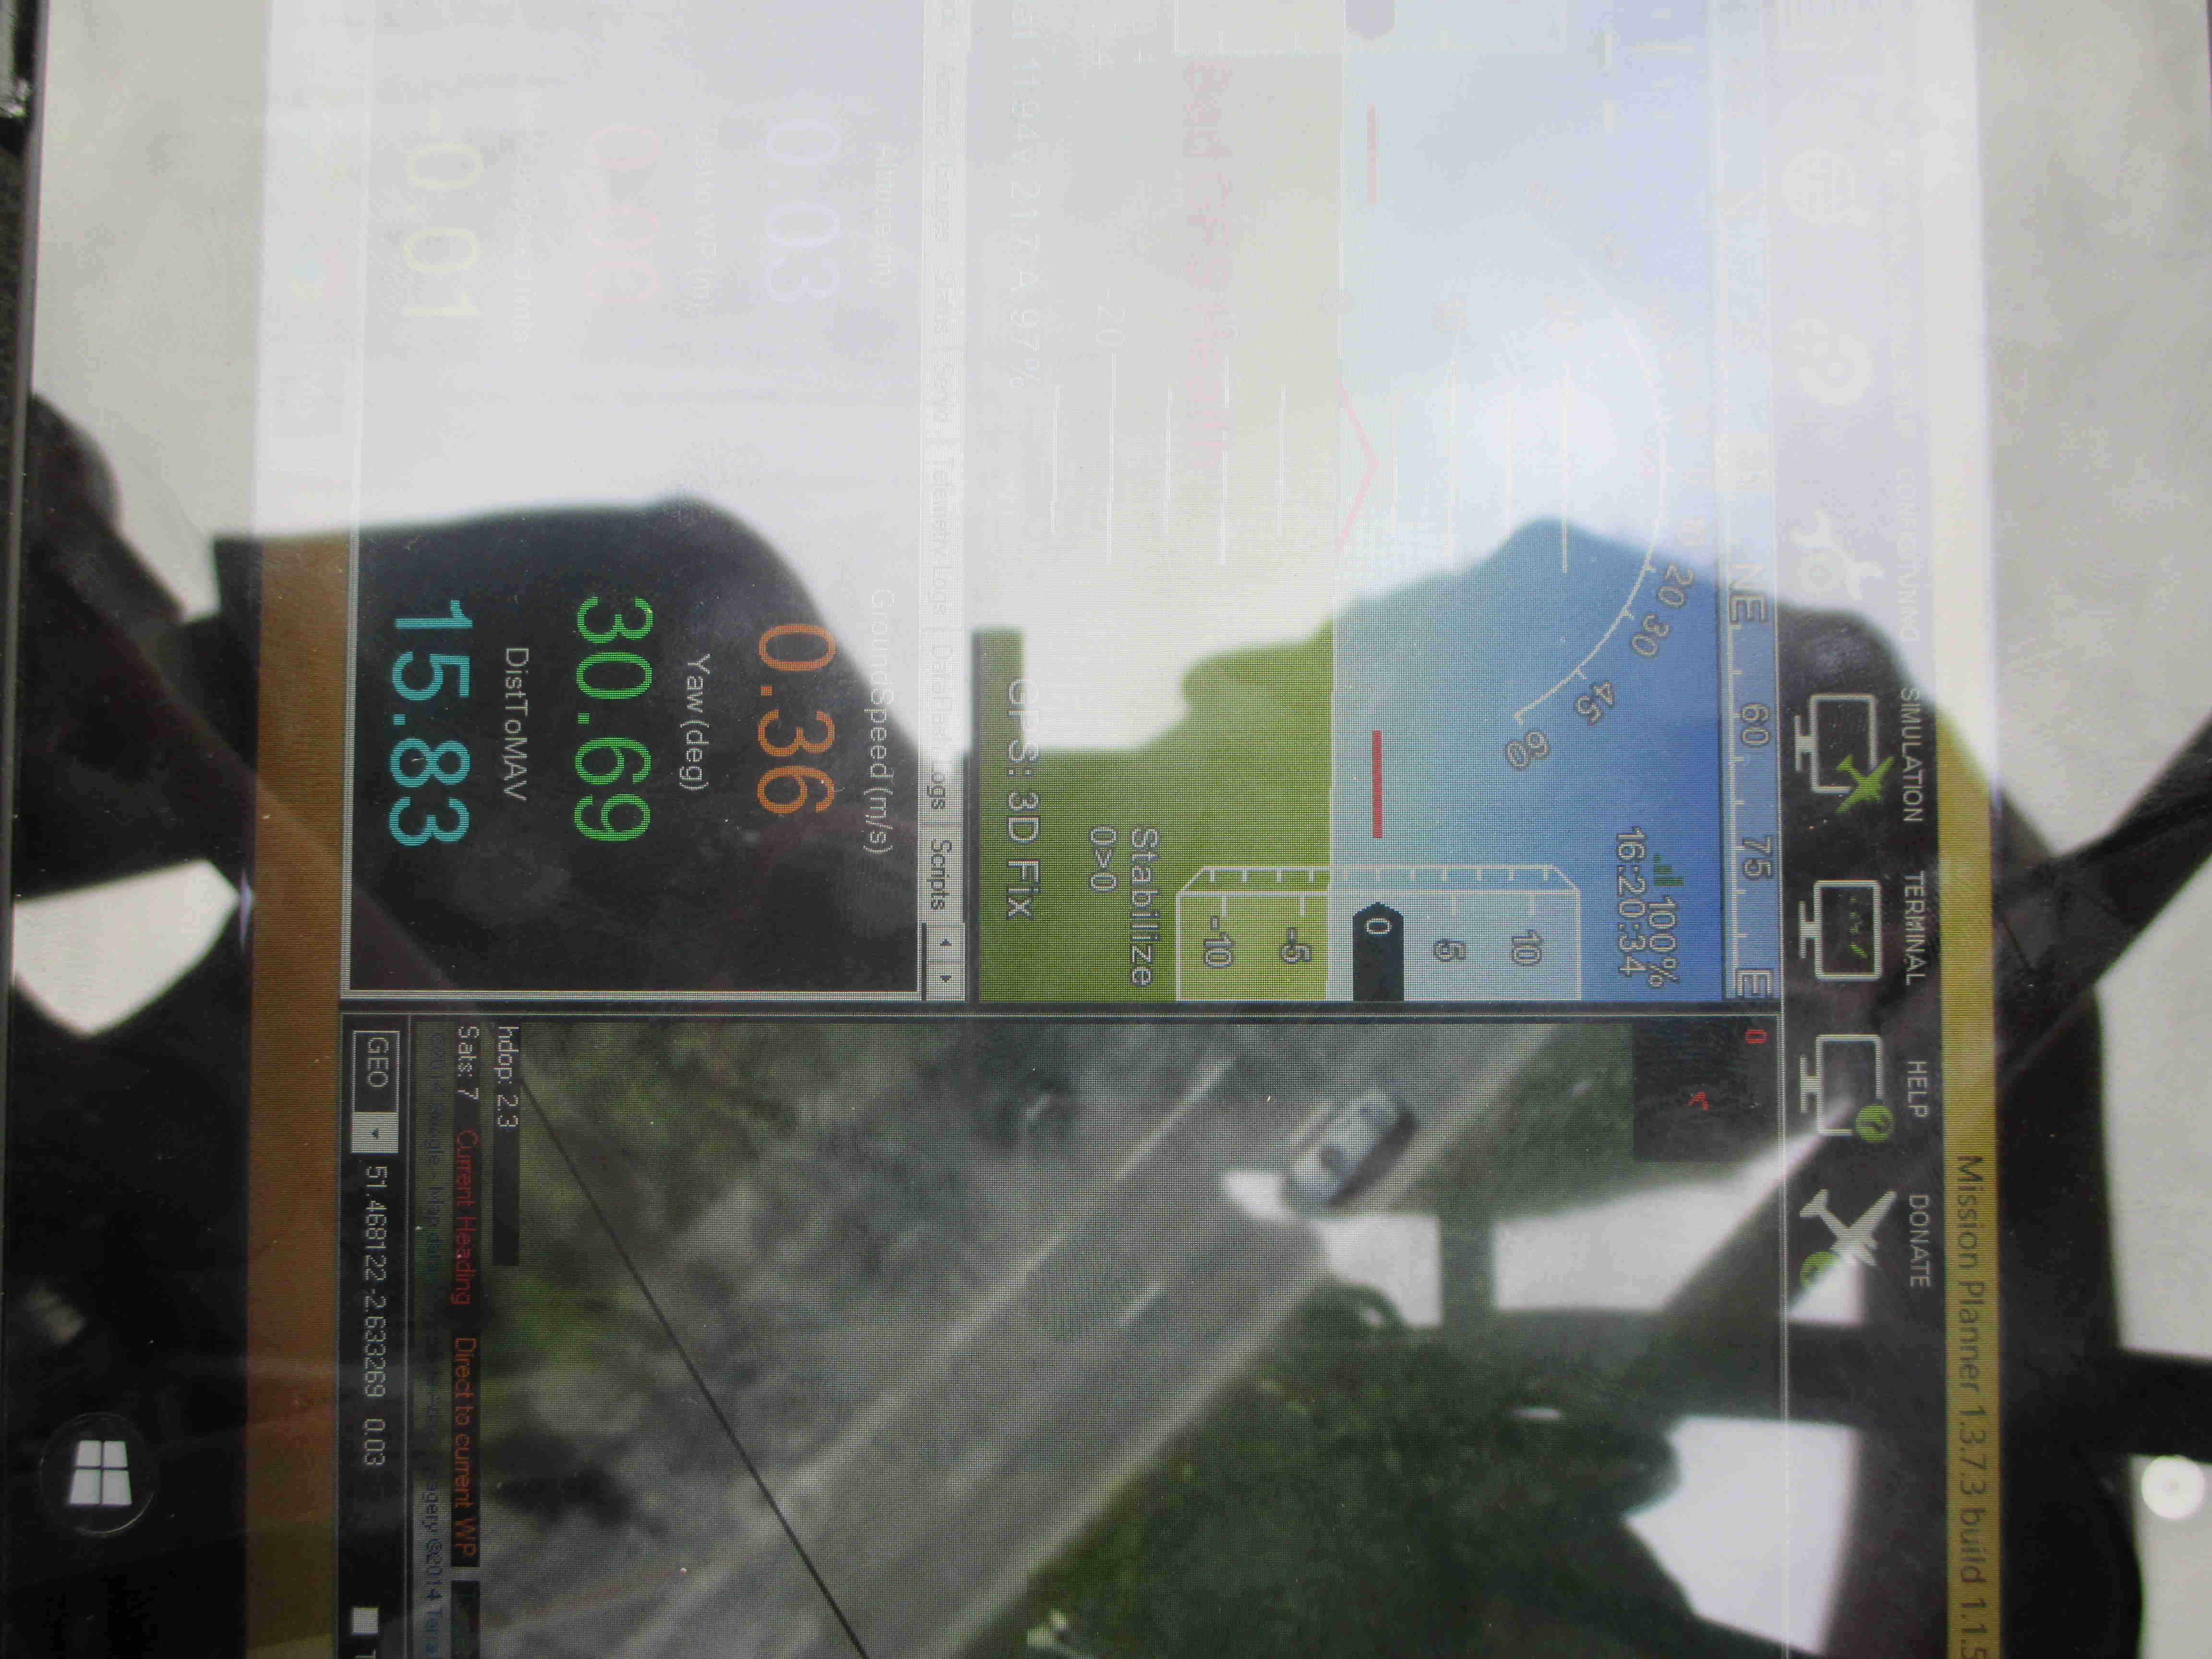
\includegraphics[width=0.5\textwidth]{MissionPlanner}
        \caption{A photograph taken of MP while connected directly to the APM,
            giving the offset between the camera time and the UAV GPS time.}
        \label{img:mission-planner}
    \end{center}
\end{wrapfigure}

\subsubsection{CAM Dataflash Log Messages}

If using the UBASIC CHDK script given in Appendix \ref{app:pwm} to allow APM to
remotely trigger camera shooting, then the GPS time, location, altitude, roll,
pitch and yaw are all logged by APM. A line will appear in the dataflash log of
the form:

\begin{minted}{python}
CAM, GPSTime, GPSWeek, Lat, Lng, Alt, Roll, Pitch, Yaw
\end{minted}

Geotagging the photos using the CAM messages embedded in the dataflash logs is
the more accurate method, as there are no uncertainties introduced by the time
logged by the camera. 

\subsubsection{Shutter Lag}

If using the CAM message method, the lag between the instruction to shoot and
the photograph being actually taken, induced by shutter lag, can cause
systematic errors in the geotagging and must be measured so that it can be taken
into account. To quantify this, we analysed the shutter lag of the Powershot
IXUS132 we are using. This involved taking a photo of a
timer\footurl{http://edwardns.com/shutterlag.html} exactly on the second, and
noting the time shown in the photograph. We calculated the shutter lag to be
\sipm{90.3}{32.0}{ms} excluding the autofocus lag, and \sipm{341}{140.3}{ms}
including the autofocus lag. As the camera is not set to autofocus using this
method of remote photography, the former value is taken as the value of
interest. As the GPS logs are made only at a frequency of \SI{5}{Hz} (or one
every \SI{200}{ms})\footnote{As per
\url{http://copter.ardupilot.com/wiki/common-geotagging-images-with-mission-planner/\#Geotag_Mode}
and \url{https://store.3drobotics.com/products/3dr-gps-ublox-with-compass}}, the
shutter lag is rounded to the nearest \SI{200}{ms} and taken as zero.

\subsection{Ground Control Points}

To enhance the accuracy and precision of the reconstructions, we employed Ground
Control Points (GCPs). These are strategically placed markers, the exact
location of which are surveyed and subsequently input into PhotoScan. Then, in
PhotoScan, after the cameras are aligned, inputting the GCPs as markers and
giving their geolocation (either preferably as WGS or possibly also as local
coordinates) allows one to optimise the alignment of the cameras, producing a
more accurate dense point cloud and therefore textured model.

Distinguishable points such as dark crosses are preferable, as they are easier
to pick out on photos when creating markers in PhotoScan, and easier for
PhotoScan to analyse and pick out the location of in each picture. I particular
crosses are effective as the exact location of the marker can be precisely set
to the centre of the cross.

As per the PhotoScan
website\footurl{http://www.agisoft.ru/wiki/PhotoScan/Tips\_and\_Tricks\#Ground\_Control},
roughly 10 GCPs are required for the completion of the georeferencing, while 15
or more GCPs are preferable for improved accuracy.

The laser-based surveying equipment used to identify the GCPs is shown in Figure
\ref{img:gcp-equipment}.

\begin{wrapfigure}{r}{0.5\textwidth}
    \begin{center}
        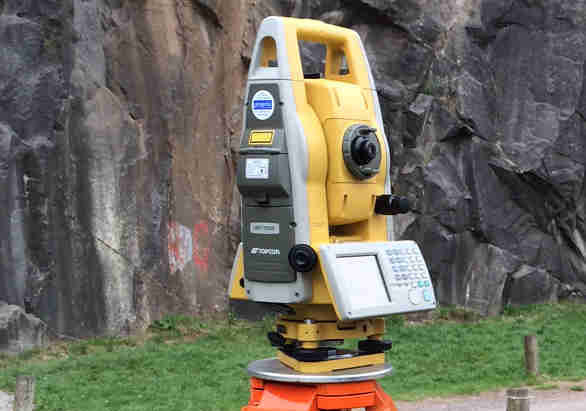
\includegraphics[width=0.5\textwidth]{GCPEquipment}
        \caption{The equipment used to survey in Ground Control Points.}
        \label{img:gcp-equipment}
    \end{center}
\end{wrapfigure}

\subsection{Accuracy and Precision Measurements}
% Should this be in methods, results or a separate theory section?

\subsubsection{Calculating the meters per pixel}

Todo

\subsubsection{Ensuring sufficient photo overlap}

Todo
